\documentclass{datest}
%\usepackage{fancyhdr}
\usepackage{wrapfig}
\usepackage{multirow}
\usepackage{array}
\usepackage{amssymb}
\usepackage{amsmath}
%\usepackage{picins}
\usepackage{floatrow}
\newfloatcommand{capbtabbox}{table}[][\FBwidth]

\usepackage{blindtext}
%\usepackage{pgfplots}

\usepackage{tikz}
\usetikzlibrary{calc,fadings,decorations.pathreplacing}
\usetikzlibrary{arrows}

\newcommand\pgfmathsinandcos[3]{%
  \pgfmathsetmacro#1{sin(#3)}%
  \pgfmathsetmacro#2{cos(#3)}%
}
\newcommand\LongitudePlane[3][current plane]{%
  \pgfmathsinandcos\sinEl\cosEl{#2} % elevation
  \pgfmathsinandcos\sint\cost{#3} % azimuth
  \tikzset{#1/.estyle={cm={\cost,\sint*\sinEl,0,\cosEl,(0,0)}}}
}
\newcommand\LatitudePlane[3][current plane]{%
  \pgfmathsinandcos\sinEl\cosEl{#2} % elevation
  \pgfmathsinandcos\sint\cost{#3} % latitude
  \pgfmathsetmacro\yshift{\cosEl*\sint}
  \tikzset{#1/.estyle={cm={\cost,0,0,\cost*\sinEl,(0,\yshift)}}} %
}
\newcommand\DrawLongitudeCircle[2][1]{
  \LongitudePlane{\angEl}{#2}
  \tikzset{current plane/.prefix style={scale=#1}}
   % angle of "visibility"
  \pgfmathsetmacro\angVis{atan(sin(#2)*cos(\angEl)/sin(\angEl))} %
  \draw[current plane] (\angVis:1) arc (\angVis:\angVis+180:1);
  \draw[current plane,dashed] (\angVis-180:1) arc (\angVis-180:\angVis:1);
}
\newcommand\DrawLatitudeCircle[2][2]{
  \LatitudePlane{\angEl}{#2}
  \tikzset{current plane/.prefix style={scale=#1}}
  \pgfmathsetmacro\sinVis{sin(#2)/cos(#2)*sin(\angEl)/cos(\angEl)}
  % angle of "visibility"
  \pgfmathsetmacro\angVis{asin(min(1,max(\sinVis,-1)))}
  \draw[current plane] (\angVis:1) arc (\angVis:-\angVis-180:1);
  \draw[current plane,dashed] (180-\angVis:1) arc (180-\angVis:\angVis:1);
}

%% document-wide tikz options and styles

\tikzset{%
  >=latex, % option for nice arrows
  inner sep=0pt,%
  outer sep=2pt,%
  mark coordinate/.style={inner sep=0pt,outer sep=0pt,minimum size=3pt,
    fill=black,circle}%
}



\usepackage{hyperref}

\hypersetup{colorlinks=true,
			urlcolor=blue,
			}
			
\usepackage{advdate}

\newcommand{\advanceday}[1][7]{%
\begingroup
\AdvanceDate[#1]%
\today%
\endgroup
}%

\newcommand{\evenmoreadvanceday}[1][28]{%
\advanceday[#1]%
}%

\newcolumntype{N}{@{}m{0pt}@{}}

  \setlength{\headheight}{30pt}
  \lhead{BCN 1210: Construction Materials \\ Concrete Homework (10 points)}
  \chead{Due on-line: \advanceday}%\today}
  \rhead{Name: \vrule height 0 pt depth 0.4 pt width 2.85 in \\ Class section: \vrule height 0 pt depth 0.4 pt width 1.25 in }

%\newcommand*{\tightlist}{\itemsep1pt \parskip0pt \parsep0pt}

\author{Damon Allen Ph.D}

%\title{BCN4423c - Timber Beam Test}
\setlength{\parindent}{0pt}
\setlength{\parskip}{0.5ex plus 0ex minus 0.2ex}
    \begin{document}
    \instruction{1}{5}{Show your calculations to receive partial credit.  Show your results to three significant digits.}
    
    \saproblem{Given the unit weight ($w_c$) of a sample of concrete is 120 $pcf$ ($lb/ft^3$) and its strength ($f'_c$) is 
    3,000 $psi$.   What is the expected Modulus of Elasticity using $E_c = w_c^{1.5} 33\sqrt{f'_c}$ ?}

\answer{$$E_c = (120 pcf)^{1.5} 33\sqrt{3,000 psi}$$
$$E_c = 2,376,000 psi$$
$$E_c = 2.38\times 10^6 psi$$}


    \saproblem{If the concrete in problem 1 had a unit weight of 145 $pcf$ what would its Modulus of Elasticity be?}

\answer{$$E_c = (145 pcf)^{1.5} 33\sqrt{3,000 psi}$$
$$E_c = 3,155,924 psi$$
$$E_c = 3.16\times 10^6 psi$$}

    \saproblem{Given a sample of normal weight concrete with a strength of 4,000  $psi$.  What would the modulus of Elasticity be using $E_c = 57,000\sqrt{f'_c}$ ?}

\answer{$$E_c = 57,000\sqrt{4,000 psi}$$
$$E_c = 3,604,997 psi$$
$$E_c = 3.60\times 10^6 psi$$}

    \saproblem{If you needed to have normal weight concrete with a Modulus of Elasticity of $3.00\times 10^6 psi$ what strength ($f'_c$) would you need? (Not what you would ask for.)}
    
\answer{
\begin{tabular}{p{6cm}|p{6cm}|p{6cm}}
$57,000\sqrt{f'_c} = E_c$&$f'_c = \left(\frac{3.00\times 10^6 psi}{57,000}\right)^2$&Rounding to the next 100 psi...\\
$f'_c = \left(\frac{E_c}{57,000}\right)^2$&$f'_c = 2,770 psi$&$f'_c = 2,800 psi$
\end{tabular}}
\vspace{0.0625in}

    \saproblem{If instead of normal weight concrete you wanted to use a light weight concrete ($w_c = 115 pcf$) but you still wanted to have a Modulus of Elasticity of $3.00\times 10^6 psi$ what strength ($f'_c$) would you need? (Not what you would ask for.)}

\answer{
\begin{tabular}{p{6cm}|p{6cm}|p{6cm}}
$w_c^{1.5} 33\sqrt{f'_c} = E_c$&$f'_c = \left(\frac{3.00\times 10^6 psi}{(115 pcf)^{1.5} 33}\right)^2$&Rounding to the next 100 psi...\\
$f'_c = \left(\frac{E_c}{w_c^{1.5} 33}\right)^2$&$f'_c = 5,434 psi$&$f'_c = 5,500 psi$
\end{tabular}}    
\vspace{0.0625in}
   
    \instruction{6}{7}{Given: A company you are working for has decided to put up a Christmas tree for the kids this year and its your job to help the children build the decorations.  Since it is a construction company the tree is going to be made from A706 rebar (the only kind to weld) and the decorations are going to be 4" diameter balls of concrete.  A special mix of light weight concrete which has a slump of practically 12" will be used to fill the clear 96 plastic molds.  To make the filling controllable a coworker brought in an old aquarium pump to fill the balls with.  The pump can supply the mixed concrete at a rate of 34.9$\frac{gal}{hr}$ (7.48052 $gal$ = 1 $ft^3$).}
    
    \saproblem{How long will it take for a single ball to be filled?}
    
    \answer{\begin{tabular}{p{4.8cm}|p{9cm}|p{6cm}}
$Vol = \frac{4}{3} \pi r^3$ & $Rate = 34.9 \frac{gal}{hr} \times \frac{1 ft^3}{7.48052 gal} \times\frac{(12")^3}{(1 ft)^3}\times\frac{1 hr}{60 min}\times\frac{1 min}{60 s}$ & $t =14.964 s$ \\
$Vol = \frac{4}{3} \pi (2")^3= 33.51 in^3$ & $Rate = 2.239 \frac{in^3}{s}$ & with 3 significant digits\\
$Rate = \frac{Vol}{t} \therefore t = \frac{Vol}{Rate}$&$t=\frac{33.51 in^3}{2.239 \frac{in^3}{s}}$ & $t = 15.0 s$
\end{tabular}}
    \vspace{0.0625in}
    
    \saproblem{What is the \underline{instantaneous} (\emph{not average}) rate of filling of a mold (\emph{change in height of the concrete}) when it has 3" for concrete in it? (FYI average rate would be found by $\frac{\text{Remaining Volume}}{\text{Remaining Fill Time}}$)}
% \newgeometry{textwidth=7in}   
 \makeatletter
 \pgfdeclareradialshading[tikz@ball]{ball}{\pgfqpoint{-20bp}{20bp}}{%
 color(0bp)=(tikz@ball!0!white);
 color(17bp)=(tikz@ball!0!white);
 color(21bp)=(tikz@ball!70!black);
 color(25bp)=(black!70);
 color(30bp)=(black!70)}
 \makeatother
 
 \setlength{\intextsep}{0.5cm}
 
%\begin{wrapfigure}[4]{L}{0.30\textwidth}  
%\begin{figure}
\vspace{-0.25in}
\begin{figure}[h]
\begin{floatrow}

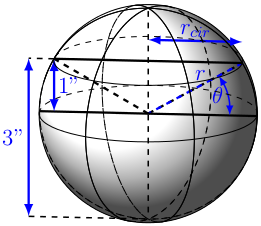
\includegraphics[width=5cm]{Sphere.png}  

%\end{figure}
%\end{wrapfigure}

%\begin{wrapfigure}{l}{0.011\textwidth}

%\end{wrapfigure}
% \vspace{-1.55in}
\capbtabbox{

\begin{tabular}{c|c}

$h_{0} = h - r = 3" - 2" = 1"$ & $Area_{cir} = \pi r_{cir}^2 $ \\
$\theta = \sin^{-1}\left(\frac{h_0}{r} \right)=\sin^{-1}\left(\frac{1"}{2"} \right)=30^\circ$ &$Area_{cir} = \pi (1.732")^2 $ \\
$r_{cir} =  r \cos(\theta) = 2" \cos(30^\circ)$ & $Area_{cir} = 9.425 in^2$\\
$r_{cir} \approx 1.732" $&$\frac{\delta h}{\delta t}  = \frac{Rate}{Area_{cir}}$
\end{tabular}

}{$\displaystyle\frac{\delta h}{\delta t}  = \frac{2.239 \frac{in^3}{s}}{9.425 in^2} =  0.238 \frac{in}{s}$}
\end{floatrow}

\end{figure}

 
% \vspace{.25in}


    
    \instruction{8}{10}{A concrete supplier that you have been using has had to switch to using aggregate from a different source, and developed a new mix design.  Since the switch was very recent your supplier has only been able to conduct 20 strength tests so far.  They provide you with the standard deviation of the 20 samples ($S_{20} = 740 psi$).  The project you are currently working on requires you to provide concrete with $f'_c$ of 3,000 $psi$ and 5,300 $psi$.  (\emph{Relevant lecture \href{http://damontallen.github.io/Construction-materials/Concrete.slides.html\#/12}{\underline{slide}} for reference.})}
 
 %  
    %\newgeometry{textwidth=7in}
    %\restoregeometry 
    
    \saproblem{What is the value of concrete strength ($f'_{cr}$) you are required to order to get $f'_c=3,000 psi$ while limiting the chance of having a batch that is too weak?}
    
    \answer{\begin{tabular}{l|c|r}
    $S = S_{20}\times 1.08 = 740 psi \times 1.08$ & \multirow{2}{*}{$f'_{cr} = \max \left\{\begin{array}{rl}f'_c +1.34 S = 4,071 psi\\f'_c +2.33 S -500 = 4,362 psi\end{array} \right. $} & $f'_{cr} = 4,362 psi$\\
    $S = 799.2 psi$& &Use: $ f'_{cr} = 4,400 psi$
    \end{tabular}}
    
\vspace{0.0625in}
    
    \saproblem{What would the value be for $f'_{cr}$ for when $f'_c=5,300 psi$? }
    
    \answer{\begin{tabular}{l|c|r}
    $S = S_{20}\times 1.08 = 740 psi \times 1.08$ & \multirow{2}{*}{$f'_{cr} = \max \left\{\begin{array}{rl}f'_c +1.34 S = 6,371 psi\\0.9 f'_c +2.33 S = 6,632 psi\end{array} \right. $} & $f'_{cr} = 6,632 psi$\\
    $S = 799.2 psi$& &Use: $ f'_{cr} = 6,700 psi$
    \end{tabular}}
    \vspace{0.0625in}
    
    \saproblem{If with further testing of 5 more samples (25 total) the standard deviation drops to $S_{25} = 400 psi$ what would the new value of $f'_{cr}$ be for when you need $f'_c=3,000 psi$?}
    
        \answer{\begin{tabular}{l|c|r}
    $S = S_{25}\times 1.03 = 400 psi \times 1.08$ & \multirow{2}{*}{$f'_{cr} = \max \left\{\begin{array}{rl}f'_c +1.34 S = 3,552 psi\\f'_c +2.33 S -500 = 3,460 psi\end{array} \right. $} & $f'_{cr} = 3,460 psi$\\
    $S = 412 psi$& &Use: $ f'_{cr} = 3,500 psi$
    \end{tabular}}
    
    \end{document}